\subsection{Расстояние и размеры}
\term{Астрономическая единица}~--- единица измерения расстояния в астрономии, 
равная большой полуоси орбиты Земли.\begin{equation}
	1~\au = 149\:597\:870\:700~\text{м} \simeq 1.5 \times 10^{11}~\text{м}
\end{equation}

\term{Годичный параллакс} ($\pi$) объекта~--- это угол, под которым видно 
орбиту Земли из окрестностей данного объекта. Применяется к объектам вне 
Солнечной системы.
\begin{equation}
\sin\pi=\frac{a_\oplus}{r},
\end{equation}
где $a_\oplus$~--- большая полуось орбиты Земли и $r$~--- расстояние до объекта 
имеют одинаковые единицы измерений. Учитывая малость угла $\pi$, можно заменить 
$\sin\pi$ на $\pi$, в результате чего получится следующее выражение для 
параллакса:\begin{equation}
	\pi = \frac{a_\oplus}{r}
\end{equation} 

\begin{figure}[h!]
\centering
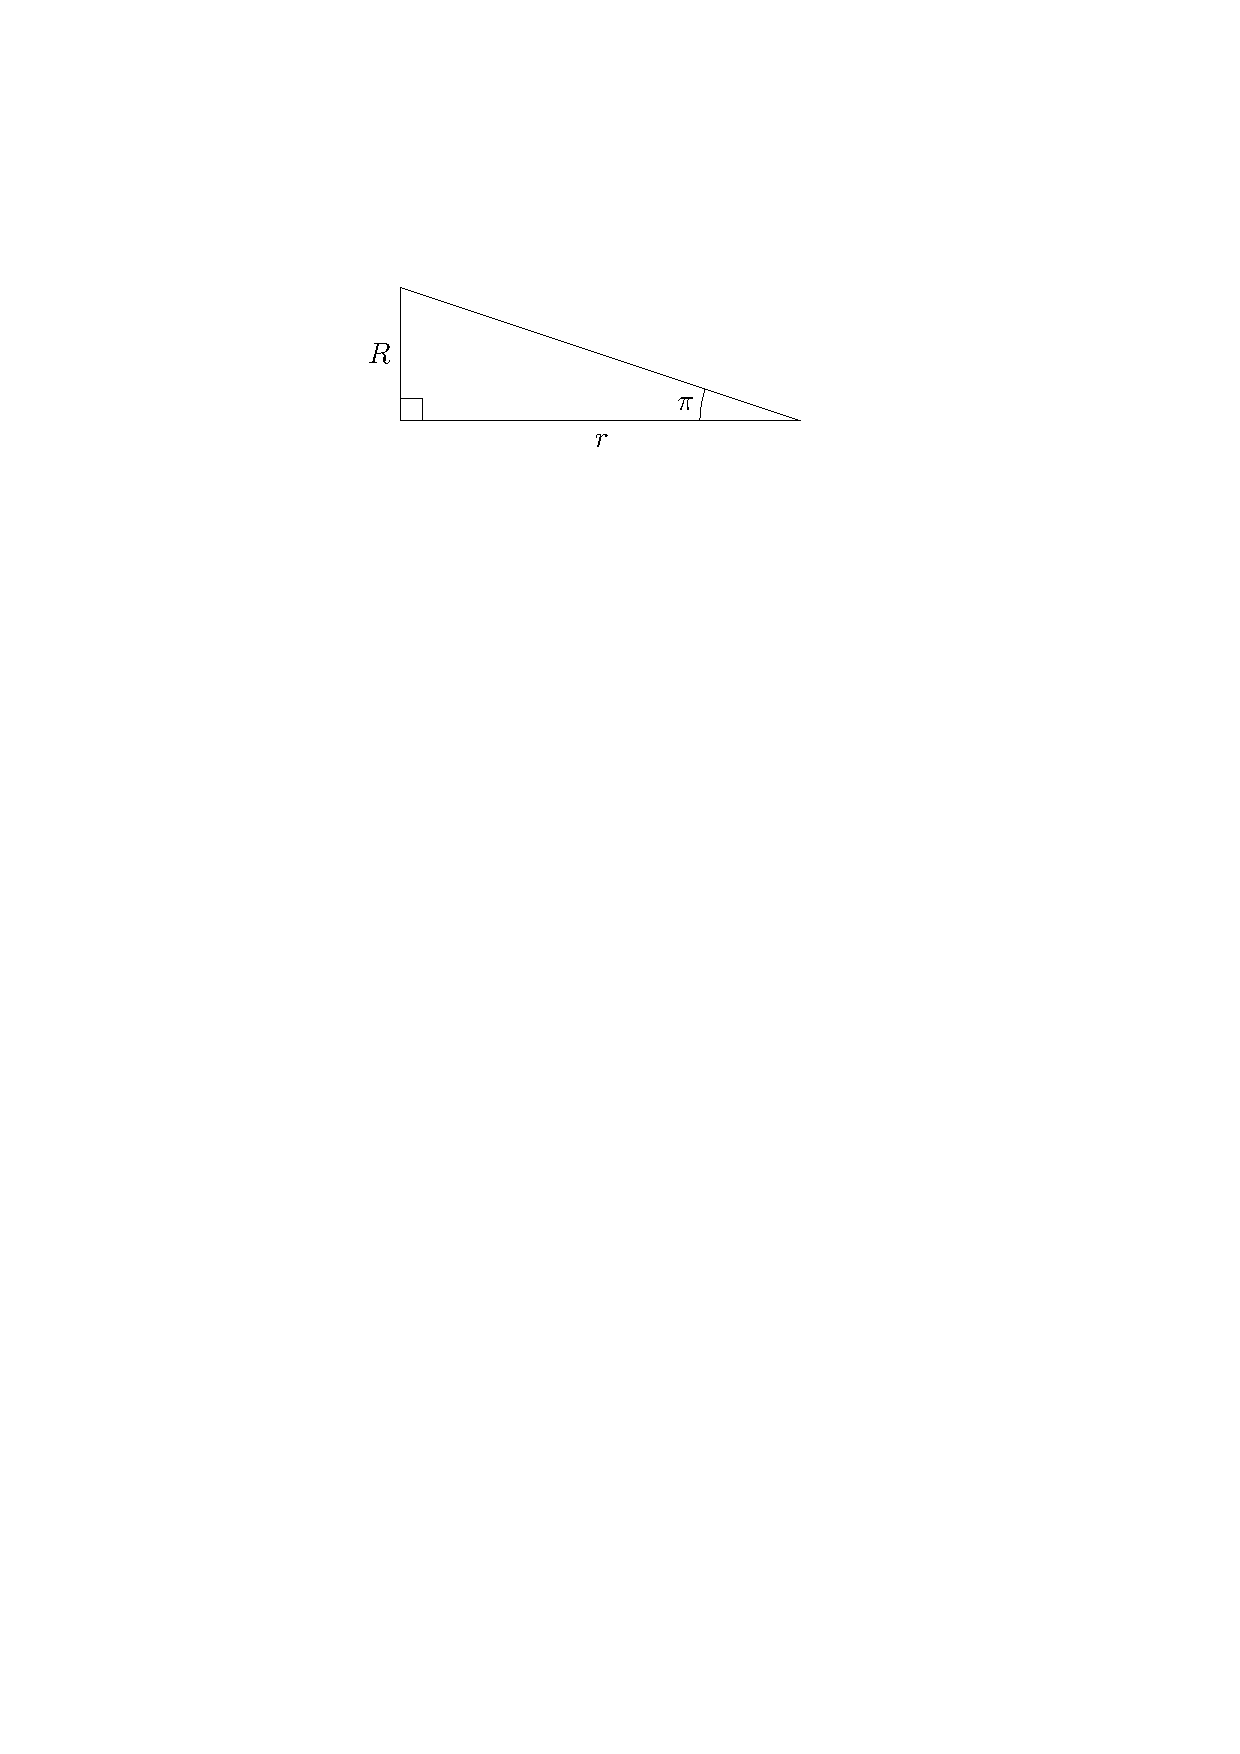
\includegraphics[width = 0.7\textwidth]{1-second}
\caption{Параллакс}
\end{figure}

Расстояние $r$, с которого большая полуось орбиты Земли $a_\oplus$ видна под 
углом $\pi = 1''$ называется \term{1 парсеком}. Так как \begin{equation}
	1~\text{рад} = \frac{180^\circ}{\pi} \simeq  3 438' \simeq 206265'' 
\quad \Longrightarrow \quad \mathsf{1~\text{\sffamily пк} = 
206265~\text{\sffamily а.\,е.}},
\end{equation} 
следовательно, записывая большую полуось орбиты Земли в \au, а расстояние до 
звезды в парсеках, получим параллакс в секундах. Таким образом, получаем 
следующую формулу:\begin{equation}
r_\text{пк}=\frac{1~\au}{\pi''},
\end{equation}
где $r$ --- расстояние до звезды (в парсеках), $\pi$ --- годичный параллакс 
звезды (в секундах).\\


\term{Угловой размер объекта} --- это угол, под которым видно диаметр объекта.
\begin{equation}
\rho =2 \arctg \left( \frac{D}{2 r} \right), 
\end{equation}
где $D$~--- диаметр объекта, а $r$~--- расстояние до него.
\begin{figure}[h!]
\centering
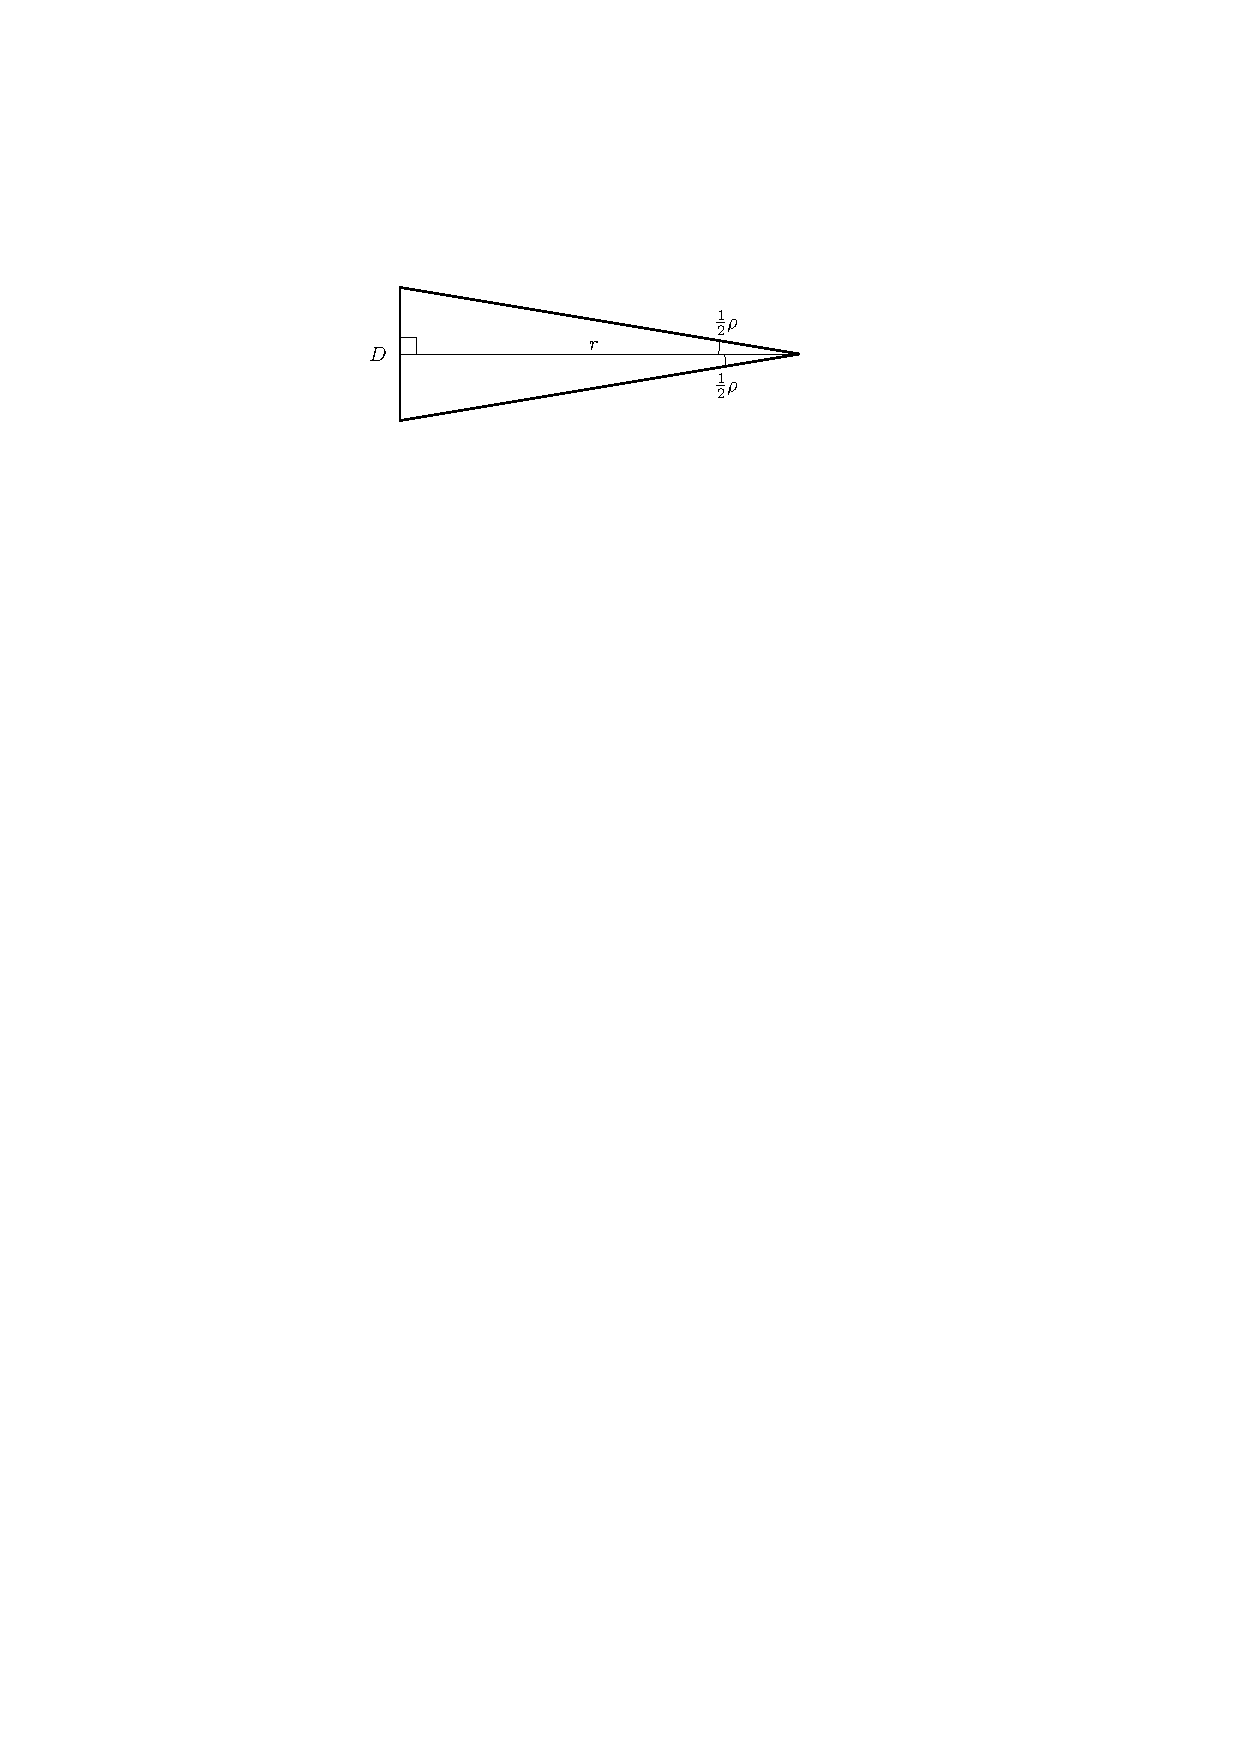
\includegraphics[width = 0.6\textwidth]{angle-size}
\caption{Угловой размер}
\end{figure}

При расстоянии $r$ много больше размера объекта $r$, то есть ($r\gg D$),
  воспользоваться приближением для малых углов: \begin{equation}
\rho \simeq \frac{D}{r}
\end{equation}

\term{Горизонтальный параллакс} --- это угол, под которым видно радиус Земли, 
при положении светила на горизонте.
\begin{equation}
\sin p=\frac{R_\oplus}{r},
\end{equation}
где $R_\oplus$ --- радиус Земли, $p$ --- горизонтальный параллакс, $r$ --- 
расстояние до объекта.\\

\begin{figure}[h!]
\centering
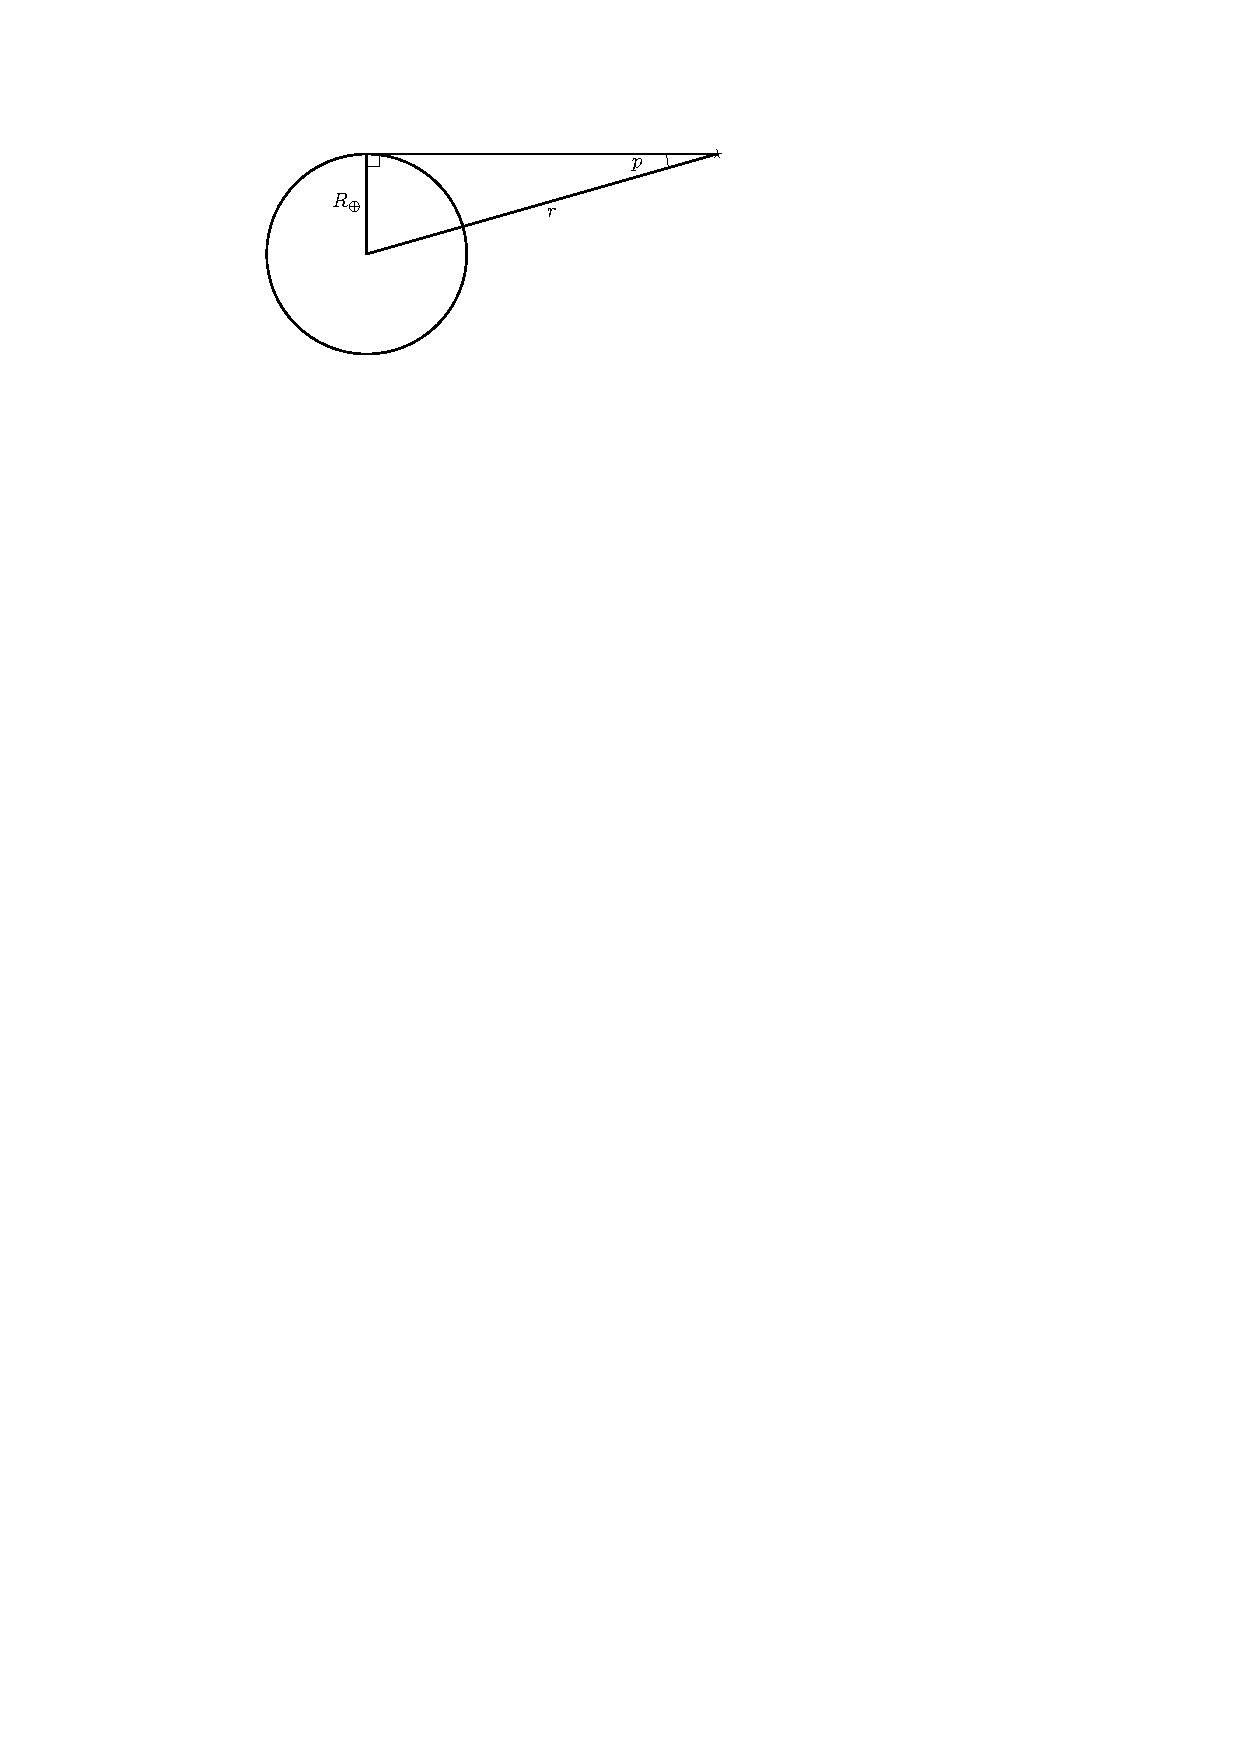
\includegraphics[width = 0.6\textwidth]{horiz-parallax}
\caption{Горизонтальный параллакс}
\end{figure}

\term{Правило Тициуса-Боде} --- эмпирическая формула приблизительно описывающая 
радиусы орбит планет от Солнца:
\begin{equation}r=\frac{3\cdot 2^n+4}{10}, \quad tn=-\infty, 0, 1, 2...
\end{equation}

